\documentclass[11pt,a4paper]{article}
\usepackage[T1]{fontenc}
\usepackage[utf8]{inputenc}
\usepackage[spanish]{babel}
\usepackage{lmodern}
\usepackage[margin=2.5cm]{geometry}
\usepackage{graphicx}
\usepackage{float}
\usepackage{tikz}
\usepackage[hidelinks]{hyperref}

% Inserta una captura si existe; si todavía no está, muestra un recuadro
\newcommand{\captura}[2]{%
  \begin{figure}[H]\centering
  \IfFileExists{#1}{\includegraphics[width=\linewidth]{#1}}%
    {\fbox{\parbox{0.9\linewidth}{\centering\vspace{2cm}Falta \texttt{\detokenize{#1}}\vspace{2cm}}}}
  \caption{#2}
  \end{figure}}

\begin{document}

% ---------------- Carátula ----------------
\begin{titlepage}
\begin{tikzpicture}[remember picture,overlay]
\draw[line width=0.5pt] ([xshift=1cm,yshift=-1cm]current page.north west)
rectangle ([xshift=-1cm,yshift=1cm]current page.south east);
\end{tikzpicture}
\centering
\vspace*{0.3cm}
\IfFileExists{evidencia/logo-uteq.jpg}{
\includegraphics[width=4.5cm]{evidencia/logo-uteq.jpg}}{}\par
\vspace{0.6cm}
{\fontsize{20}{24}\selectfont\bfseries UNIVERSIDAD TÉCNICA ESTATAL\\DE QUEVEDO\par}
\vspace{0.4cm}
{\large\bfseries FACULTAD DE CIENCIAS DE LA COMPUTACIÓN\par}
{\itshape CARRERA INGENIERÍA EN SOFTWARE\par}
\vspace{0.8cm}
{\bfseries APLICACIONES DISTRIBUIDAS\par}
{\bfseries Séptimo nivel -- Paralelo B\par}
\vspace{0.7cm}
{\large\bfseries EV -- Unidad I -- Aporte Parte Práctica\\[2pt]
Examen práctico: BoletoDistribuido\par}
\vspace{0.7cm}
PRESENTADO POR:\par
\vspace{0.2cm}
{\large\bfseries ZAMBRANO YONG ANGEL DANIEL\par}
\vspace{0.5cm}
{\bfseries GitHub:\par}
\href{https://github.com/iMouraad/AP-U1-Zambrano-Angel}{\texttt{https://github.com/iMouraad/AP-U1-Zambrano-Angel}}\par
\vspace{0.5cm}
Docente: Gleiston Cicerón Guerrero Ulloa, PhD\par
\vspace{0.3cm}
Fecha del examen: 23 de noviembre de 2026\par
\vspace{0.3cm}
Periodo académico: SPA 2026--2027\par
\end{titlepage}

% ---------------- Problema ----------------
\section{Problema}
En el examen me tocó construir BoletoDistribuido, un sistema de venta de
boletos que corre en tres oficinas a la vez: Quevedo, Buena Fe y Valencia.
Cada oficina es un proceso aparte, guarda su propia copia de los asientos
vendidos y puede atender a un cliente. Lo que no se puede permitir es vender
dos veces el mismo asiento, ni cuando dos oficinas lo piden al mismo tiempo
ni cuando una de ellas se cae a mitad de la venta.

\section{Solución implementada}
Puse todo en un solo archivo, \texttt{boleto.py}. Cada oficina la levanto
con \texttt{python boleto.py nodo N}: Quevedo escucha en el puerto 6001,
Buena Fe en el 6002 y Valencia en el 6003.

\subsection{Mensajes delimitados y token}
Hice que los nodos se comuniquen por sockets TCP. Cada mensaje lo mando
como un JSON que termina en salto de línea, y del otro lado leo hasta ese
salto para saber dónde acaba. A todos los mensajes les agrego el campo \texttt{token} con
\texttt{uteq-2026}. Si llega uno con otro token, el nodo contesta
\texttt{token inválido} y no lo procesa.

\subsection{Lamport con orden total}
Cada nodo lleva su reloj lógico. Antes de enviar lo subo en 1 y lo mando en
el campo \texttt{lamport}; cuando recibo, me quedo con el mayor entre mi
reloj y el que llegó, y le sumo 1. Tomé en cuenta que dos nodos pueden
quedar con el mismo valor, así que para el orden total uso el par
\texttt{(reloj, id)}: si empatan, va primero el de id menor. Por eso cada
línea del registro sale como \texttt{L=(reloj,id)}. Como el reloj lo tocan
varios hilos, lo cambio siempre dentro de un \texttt{Lock}.

\subsection{Latidos}
Hice que cada nodo que no es coordinador le mande un \texttt{LATIDO} al
coordinador cada segundo. Si fallan tres seguidos, lo doy por caído y ese
nodo arranca una elección.

\subsection{Bully}
Programé la elección para que el nodo que la empieza solo les escriba a
los que tienen id mayor. Si alguno contesta, se hace a un lado y espera; si
nadie contesta, se declara coordinador y se lo avisa al resto con un
mensaje \texttt{COORDINADOR}. Dejé a Valencia, el nodo 3, como coordinador
inicial por tener el id más alto.

\subsection{2PC}
La oficina que recibe una venta se la pasa al coordinador. En el
coordinador usé
\texttt{lock\_venta} para que el coordinador atienda las ventas de una en
una, y el commit en dos fases. Primero manda \texttt{PREPARAR}: cada nodo
vota SI y deja el asiento bloqueado, o vota NO si ya lo tiene vendido o
bloqueado. Si los tres votan SI, manda \texttt{CONFIRMAR}; con cualquier
otro resultado manda \texttt{ABORTAR}. Decidí que un nodo que no responde
cuente como \texttt{CAIDO}, y eso basta para abortar.

\begin{verbatim}
decision = ("CONFIRMAR"
            if all(v == "SI" for v in votos.values())
            else "ABORTAR")
\end{verbatim}

% ---------------- Escenarios ----------------
\section{Escenarios}

\subsection{Escenario 1: venta normal}
\captura{evidencia/evidencia-practica.png}{Venta del asiento 12 desde Quevedo}
Prendí los tres nodos y vendí el asiento 12 desde Quevedo con
\texttt{python boleto.py vender 6001 12}. Como Quevedo no era el
coordinador, le pasó la venta a Valencia, que abrió la transacción
\texttt{3-2984}. Los tres votaron SI, la decisión fue CONFIRMAR y cada nodo
dejó registrado el asiento 12 como vendido por Quevedo.

Me llamó la atención que el reloj ya fuera por 2984 con una sola venta. La
razón es que cada latido es un mensaje y mueve el reloj; con los nodos
prendidos varios minutos, los latidos de Quevedo y Buena Fe hacia Valencia
lo fueron subiendo. Al inicio de la captura también se ve que cada nodo,
como todavía no encontraba a los otros, empezó su propia elección. Al final
los tres quedaron con Valencia de coordinador.

\subsection{Escenario 2: venta simultánea del mismo asiento}
Este escenario y los siguientes los corrí después del examen, con el mismo
\texttt{boleto.py} que está en el repositorio.

\captura{evidencia/evidenciaescenario-2-original-nodos.png}{Nodos con el boleto.py del examen}
\captura{evidencia/evidenciaescenario-2-original.png}{Venta simultánea con el boleto.py del examen}
Primero lo probé con el \texttt{boleto.py} del examen y lancé a la vez la
venta del asiento 20 desde Quevedo y desde Buena Fe. A Buena Fe le
abortaron la venta con Quevedo marcado como CAIDO, y la de Quevedo terminó
en \texttt{ConnectionResetError}. Revisé el código y encontré la causa: en
\texttt{PREPARAR}, el nodo toma \texttt{self.lock} y, sin soltarlo, llama a
\texttt{log()}, que pide el mismo lock. Como \texttt{threading.Lock} no
deja que un hilo lo tome dos veces, ese hilo se queda esperando para
siempre y el nodo deja de responder.

\captura{evidencia/evidenciaescenario-2-nodos.png}{Nodos con boleto\_corregido.py}
\captura{evidencia/evidenciaescenario-2.png}{Venta simultánea con boleto\_corregido.py}
Para comprobarlo hice una copia, \texttt{boleto\_corregido.py}, en la que
solo cambié \texttt{threading.Lock()} por \texttt{threading.RLock()}, que sí
deja que el mismo hilo lo tome dos veces. Con esa versión lancé las dos
ventas otra vez. Quevedo llegó primero y su transacción \texttt{3-173} se
confirmó con los tres votos en SI. La de Buena Fe, \texttt{3-192}, recibió
tres NO porque el asiento ya estaba vendido y se abortó, así que el asiento
20 quedó vendido una sola vez.

\subsection{Escenario 3: caída del coordinador}
\captura{evidencia/escenario-3.png}{Caída de Valencia y elección de Buena Fe}
Con los tres nodos de \texttt{boleto\_corregido.py} corriendo, cerré
Valencia con Ctrl+C. Quevedo perdió tres latidos seguidos (de L=666 a
L=668) y empezó la elección. Buena Fe recibió el aviso, nadie con id mayor
le contestó y se declaró coordinador en L=672; Quevedo se enteró en L=675.
Lancé la venta del asiento 31 justo en ese momento. Quevedo todavía tenía a
Valencia como coordinador, no pudo conectarse y le devolvió al cliente
\emph{coordinador caído, reintente tras la elección}.

\captura{evidencia/escenario-3b.png}{Venta después de la elección}
Cuando terminó la elección, reintenté con el asiento 32. Esta vez la venta
la coordinó Buena Fe, por eso la transacción es \texttt{2-904}. Quevedo y
Buena Fe votaron SI, pero Valencia salió como CAIDO y la venta se abortó.
Con mi 2PC hacen falta los tres votos, así que mientras Valencia esté caído
no se puede vender ningún asiento, aunque ya haya un coordinador nuevo.

\subsection{Escenario 4: mensaje con token inválido}
\captura{evidencia/escenario-4.png}{Mensaje con token falso}
Para probar el token no toqué el código: mandé desde la terminal, con una
línea de Python, un mensaje \texttt{ESTADO} a Quevedo con el token
\texttt{falso}. El nodo respondió \texttt{token inválido} y no procesó la
petición. El \verb|á| que se ve en la respuesta es la letra á escrita
en el formato de JSON.

\captura{evidencia/escenario-4b.png}{El mismo pedido con el token correcto}
Con el token correcto, Quevedo sí devolvió su estado: coordinador 2 y el
asiento 30 vendido. El asiento 20 del escenario 2 ya no aparece porque
entre una prueba y otra reinicié los nodos, y mi sistema guarda los
vendidos solo en memoria. Si se apagan las tres oficinas, se pierden las
ventas.

\subsection{Escenario 5: caída de una oficina que no es coordinador}
\captura{evidencia/escenario-5.png}{Venta con Quevedo caído}
Levanté otra vez los tres nodos y cerré solo Quevedo. Después vendí el
asiento 40 desde Buena Fe. Valencia, que seguía de coordinador, abrió la
transacción \texttt{3-391}: Buena Fe y Valencia votaron SI y Quevedo salió
como CAIDO, así que la decisión fue ABORTAR. En el registro de Valencia
quedó \emph{nodo 1 no recibió ABORTAR}, y Buena Fe liberó el asiento que
había bloqueado. No hubo elección, porque el que se cayó no era el
coordinador.

\subsection{Escenario 6: un nodo que arranca tarde}
\captura{evidencia/evidencianodo-tarde.png}{Valencia arranca después que los otros dos}
Este caso me salió sin buscarlo, con el \texttt{boleto.py} original.
Levanté Quevedo y Buena Fe antes que Valencia. Como el nodo 3 todavía no
existía, los dos perdieron los latidos y empezaron una elección: Quevedo
alcanzó a declararse coordinador, pero Buena Fe tiene el id mayor, ganó y
se lo avisó. Cuando por fin levanté Valencia, arrancó creyéndose
coordinador, y como el coordinador no manda latidos, nunca se enteró de la
elección. Quedaron dos coordinadores: Quevedo y Buena Fe con el nodo 2, y
Valencia consigo mismo. Mi Bully no cubre el caso de un nodo que se une
tarde, porque al arrancar no llama a elección. La versión corregida tiene
el mismo comportamiento, ya que solo le cambié el lock.

% ---------------- Preguntas ----------------
\section{Preguntas de análisis}

\subsection{CAP}
En mi sistema elegí la consistencia antes que la disponibilidad. Para
vender un asiento necesito el SI de los tres nodos, y si uno no responde su
voto cuenta como \texttt{CAIDO} y la venta se aborta. Así las tres oficinas
nunca quedan con datos distintos, pero mientras un nodo esté caído o
aislado por la red no se vende nada. Ante una partición, entonces, el
sistema se porta como CP.

\subsection{Transparencias}
El cliente le pide la venta a su oficina y no tiene que saber quién es el
coordinador, porque el nodo reenvía la petición por su cuenta; eso es
transparencia de ubicación. Si dos ventas llegan a la vez, el
\texttt{lock\_venta} y el 2PC las ordenan sin que el cliente haga nada, y
como cada oficina guarda su copia de los vendidos, el cliente ve un solo
sistema aunque haya tres réplicas. Con los fallos me quedé a medias: si se
cae el coordinador, el cliente recibe \emph{coordinador caído, reintente tras
la elección}, así que se entera y tiene que volver a intentar.

\subsection{Falacias de la computación distribuida}
No supuse que la red fuera confiable. Todas las llamadas tienen timeout y
los latidos están justamente para notar cuando un nodo deja de contestar.
Tampoco supuse latencia cero, por eso usé esperas de 1, 2 y 8 segundos
según el mensaje, y tomé en cuenta que el coordinador puede cambiar con
Bully. La que dejé abierta es la de que la red es segura: el token va en
texto plano dentro del JSON, y cualquiera que capture el tráfico lo puede
leer y reutilizar.

\subsection{Bloqueo de 2PC}
Si el coordinador se cae después de mandar \texttt{PREPARAR} y antes de
mandar la decisión, los nodos que votaron SI se quedan con el asiento en
\texttt{bloqueados}. No le puse un tiempo límite que lo libere, así que ese
asiento queda trabado hasta resolverlo a mano. Ningún participante puede
decidir por su cuenta, porque no sabe qué votaron los otros. Para
arreglarlo usaría tres fases, o guardaría la decisión en un registro que el
nuevo coordinador pueda leer.

\subsection{SLA del 99,5\,\%}
Con un SLA de 99,5\,\% el sistema puede estar caído el 0,5\,\% del tiempo,
que son unas 43,8 horas al año, unas 3,6 horas en un mes de 30 días o unos
7,2 minutos al día. La caída del coordinador no se come mucho de eso: los
latidos la detectan en unos 3 segundos y la elección termina poco después.
Lo que más pesa es lo que conté en CAP. Si cualquiera de los tres nodos
está caído no hay ventas, así que la disponibilidad depende de que los tres
estén arriba al mismo tiempo.

\subsection{Límites de Lamport}
Con Lamport, si un evento causó a otro, el primero tiene un reloj menor. Al
revés no funciona: un reloj menor no prueba que haya causa, y no hay forma
de saber si dos eventos fueron concurrentes. El desempate por id que puse
da un orden total, pero ese orden lo decidí yo por convención. Tampoco mide
tiempo real: en el escenario 1 el reloj llegó a casi 3000 solo por los
latidos, y ese número no dice cuántos segundos pasaron. Para detectar
concurrencia tendría que usar un reloj vectorial.

% ---------------- Declaración de IA ----------------
\section{Declaración de uso de inteligencia artificial}
El código de boleto.py lo escribí durante el examen, sin internet y sin IA, y quedó
sin cambios. Las capturas y el texto de este informe los hice yo. Después del examen
usé Claude (Anthropic) para armar la plantilla de \LaTeX{} y para analizar mi código;
de ese análisis salió boleto\_corregido.py, una copia aparte donde cambié Lock por
RLock para probar los escenarios 2 a 5.

% ---------------- Captura del cuestionario (obligatoria, última página) -------
\clearpage
\section*{Resumen del cuestionario}
\begin{center}
\IfFileExists{evidencia/resumen-cuestionario.png}%
  {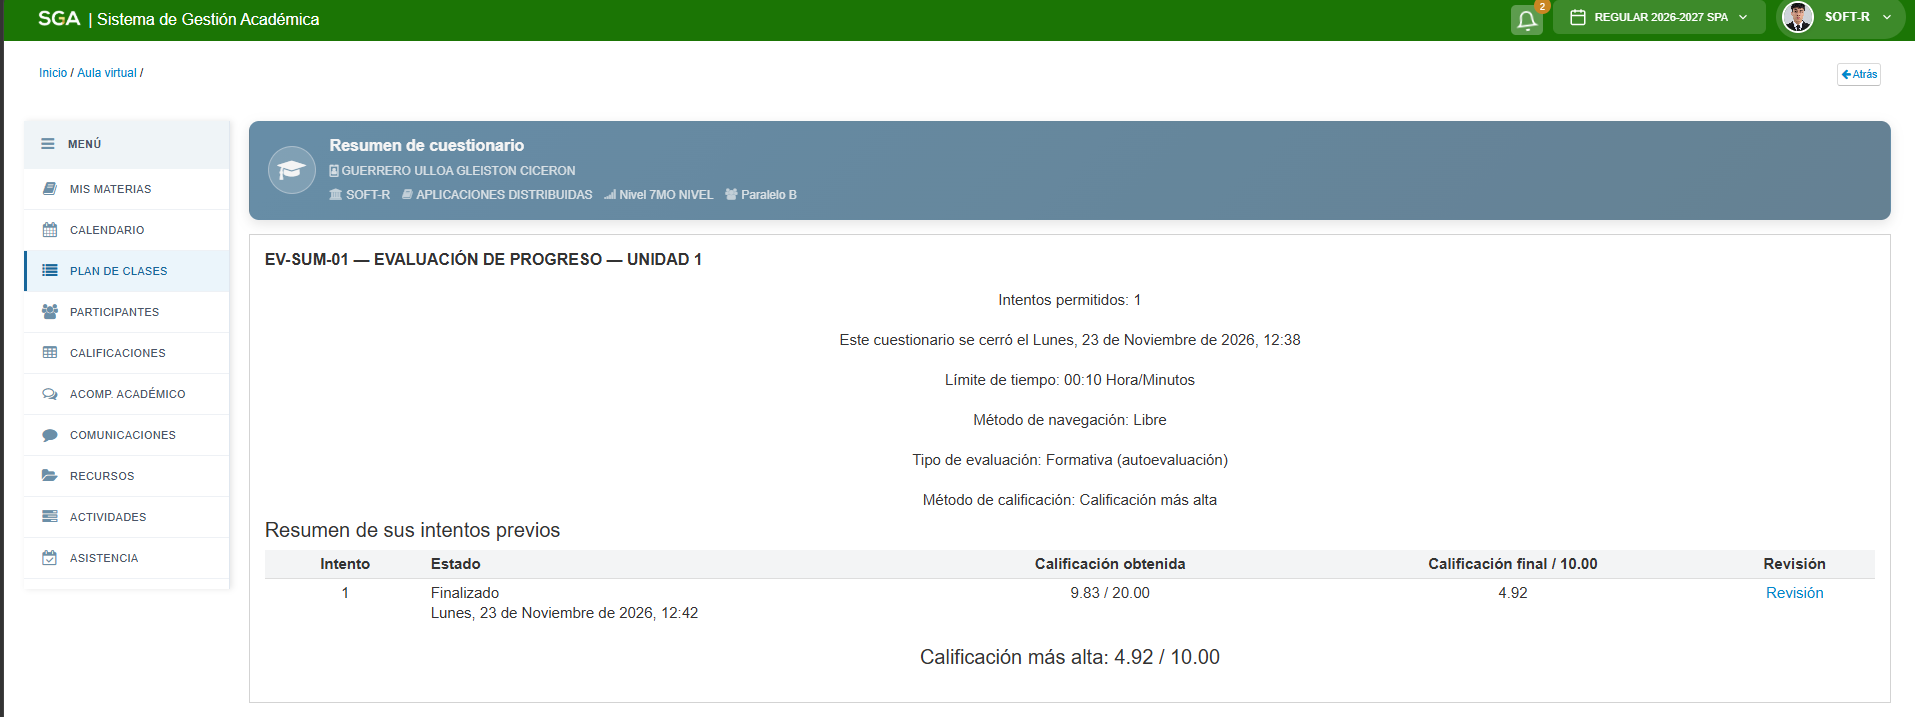
\includegraphics[width=\linewidth,height=0.85\textheight,keepaspectratio]{evidencia/resumen-cuestionario.png}}%
  {\fbox{\parbox{0.9\linewidth}{\centering\vspace{3cm}Falta \texttt{evidencia/resumen-cuestionario.png}\vspace{3cm}}}}
\end{center}

\end{document}